% tGISguide.tex
% v3.4 released April 2009

\documentclass[]{tGIS2e}
% line numbers
\usepackage[right]{lineno}

%\citestyle{tGIS}


\begin{document}

%\doi{10.1080/1365881YYxxxxxxxx}
%\issn{1362-3087} \issnp{1365-8816} \jvol{00} \jnum{00} \jyear{2009} %\jmonth{February}

%\markboth{Taylor \& Francis and I.T. Consultant}{International Journal of Geographical Information Science}

\articletype{RESEARCH ARTICLE}

\title{{\itshape Delineate urban boundaries in Great Britain from the network of Twitter user spatial interactions} }
\maketitle

\begin{abstract}
Urban regions are discrete urban areas with various socio-economic relationships and citizen commute patterns.
Defining the boundaries of urban regions is important to city planning, traffic management and resource allocation.
Existing urban boundaries are usually defined by government political and administrative purposes, however, it is not clear whether the boundaries truly reflect people's daily interactions with the urban space in their intra- and inter regional activities.
In this study, we presented a method to redraw urban boundaries based upon human interaction with the physical space.
Specifically, we delineated the urban boundaries of Great Britain using a spatial Twitter user interaction network that was inferred from over 69 million Twitter messages.
Our study connects human mobility research with the delineation of non-administrative anthropographic urban boundaries based on Twitter user spatial interactions, which provides a new understanding of the interactions between urban structure and human activity.
We redrew the non-administrative anthropographic boundaries in a hierarchical fashion based on different physical movement ranges of users inferred from the collective mobility patterns of Twitter users in Great Britain.
The result of strongly connected urban regions in the form of communities in the network space yield geographically cohesive, non-overlapping urban areas that provides a clear delineation of the non-administrative anthropographic urban boundaries of Great Britain.
The technique was applied to both national scale (Great Britain) and municipal scale (the London metropolis). 
While our results corresponded well to the administrative boundaries, many unexpected and interesting boundaries were identified.
\newline

\noindent{\bf{Keywords:}} mobility pattern, urban boundary, spatial interaction, spatial network, community structure
\end{abstract}
\linenumbers
\section{Introduction}
\markboth{International Journal of Geographical Information Science}{International Journal of Geographical Information Science}
Official urban boundaries are defined by government agencies for political and administrative purposes.
Urban environments are conceptualized as spaces that are recreated and formed by human activities~\citep{schliephake}.
A fundamental question when using the administrative, ``top-down'', approach to defining urban boundaries is whether the outcome reflects the spatial interactions of humans.
These interactions can take the form of trade, commerce, social connections, and political activity across the borders.
Urban boundaries that respect the human interaction space can be very import to city planning, traffic management and resource allocation~\citep{lynch1960,jiang2015,liu2015,long2015}.
Many studies adopt a ``bottom-up'' approach to urban boundary delineation, where the geographic space is partitioned into small units and each unit is modeled as a node within a network structure.
A suitable community detection algorithm is applied to partition the network and associated geographic space based on the strength of human interaction among the nodes~\cite{lancichinetti2009}.
Different social and physical human interactions were considered to establish the edges of the network connecting the nodes.
For example, a large set of telephone call records were used to represent the network of human interaction across space to delineate urban boundaries in Great Britain~\cite{ratti2010}.
Extending the previous method to different countries~\cite{sobolevsky2013}, the authors argue that this method yields cohesive geographic divisions that follow the socio-economic boundaries.
While other researchers use social ties of Twitter users to identify cohesive regions for different countries across the world~\cite{kallus2015}, they found evidence for dividing the urban space due to local conflicts and cross-country unifying trends that further support the ``bottom-up" approach to mapping non-administrative anthropographic boundaries.

In this study, we describe a novel approach to delineating urban boundaries based on the movements of 
Twitter users extracted from more than 69 million Twitter messages from June $1^{st}$ to December $31^{st}$, 2014.
Geo-located Twitter data is proven to be a useful source for studying human mobility patterns at large spatial scales (e.g. the country level)~\cite{hawelka,jurdak2015}.
We argue here that Twitter user mobility patterns provide a different view of non-administrative units based on physical commutes rather than social ties or phone call initiation. 
A unique advantage is that non-administrative anthropographic urban boundaries can be delineated in a hierarchical fashion based upon different ranges of physical movement, which are inferred from the collective mobility patterns of Twitter users in Great Britain. 
In addition, Twitter data are not as sensitive to user privacy issues and do not exhibit spatial granularity that is limited to the postal code level~\cite{thiemann}. 

We delineated the geography of urban boundaries in Great Britain by imposing a virtual fishnet over the islands of Great Britain.
Twitter user movements were used to establish the connections between the fishnet's cells to form a connectivity network, where each cell acts as a node within the network.
We applied the map equation algorithm~\citep{domenico2015} to partition the network and associate geographic regions.
The map equation algorithm was selected to avoid the inherent resolution problem~\cite{fortunato2007} of the common modularity maximization method~\citep{newman2006}. 
We found that the collective mobility patterns of Twitter users in Great Britain are divided into several distance ranges starting from short, intra- to inter-city movements with clear distinction points. 
The identification of connected regions at each of these distance ranges yielded hierarchical boundaries of the urban space in Great Britain.
Our study provides a first step in connecting human mobility research with the definition of non-administrative anthropographic urban boundaries based on Twitter user spatial interaction. 
It provides a new understanding of the interactions between human activity and urban structures. 

\section{Materials and Methods}
\subsection{Overview}
We use large-scale Twitter user spatial interactions inferred from the collective mobility patterns of Twitter users to delineate urban boundaries in Great Britain.
A Twitter user's movement is defined here as the individual's geographic relocation or displacement~\cite{gonzalez2008}.
This is not equivalent to a ``trip" taken by an individual, because, displacement includes situations when the time interval between two recorded locations is one month.
To identify the clusters of urban regional connectedness using large-scale Twitter data, we first imposed a virtual fishnet over the islands of Great Britain.
Twitter user movements were then used to establish the connectivity between fishnet cells to form a connectivity network where each cell is considered a node within the network. 
Finally, by detecting strongly connected clusters in the network space using community detection methods~\cite{coscia2011}, we were able to reveal urban boundaries within the geographic space. 
An overview of the approach is illustrated in Fig.~\ref{S1_Fig} and the details are presented in the following sections. 

%\begin{figure}[ht]
%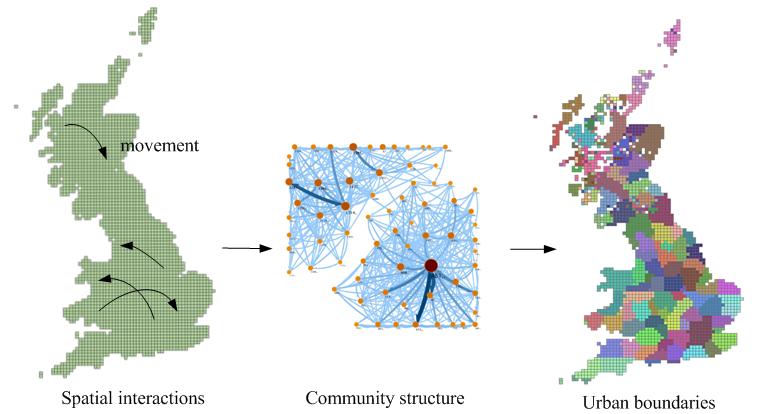
\includegraphics[width=1\linewidth]{./figure/S1_overview_Fig_2}
%\caption{{\bf An overview for delineating urban boundaries from Twitter user movements}}
%\label{S1_Fig}
%\end{figure}

\begin{figure}[ht]
\begin{center}
\vspace{36pt}
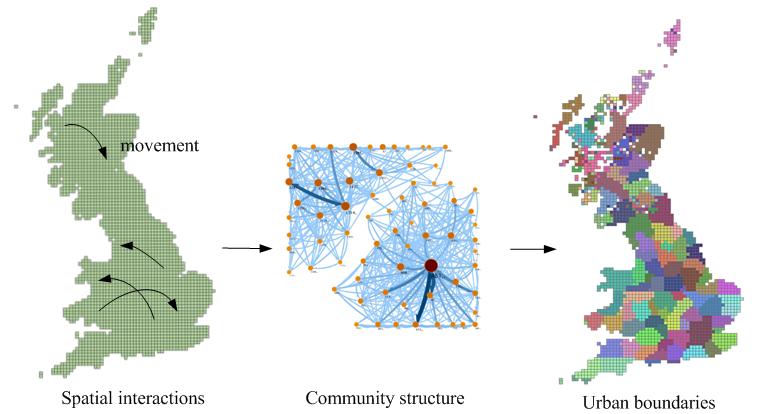
\includegraphics[width=1\linewidth]{./figure/S1_overview_Fig_2}
\caption{\bfseries{An overview for delineating urban boundaries from Twitter user movements}}
\label{S1_Fig}
\end{center}
\end{figure}

\subsection{Geo-located Twitter Data}
A geo-located tweet is a Twitter message with an additional geo-tag expressed as a pair of geographical coordinates that represent the location from which the tweet was sent.
For this study, geo-located tweets were collected using the Twitter Streaming API (
{\tt{https://dev.twitter.com/streaming/overview}}) by supplying a geographical bounding box to retrieve all the  geo-located tweets within an area of interest. To ensure complete coverage of Great Britain, we set the bounding box to the British Isles using the lower left and upper right coordinates (49.497, -14.854), (61.186, 2.637) respectively. This does include the whole of Ireland part of France.
We implemented a data crawler to continuously collect 7-months of data (June $1^{st}$ -- December $31^{st}$, 2014) resulting in over 101.8 million tweets with a total data volume of 60 GB, which we restrict to 69 million based on a process outlined below. 
To showcase the overall spatial coverage of the collected geo-located tweets, a density map of the tweet locations in British Isles for July 2014 is shown in Fig.~\ref{S2_Fig}.
The collected point visualization reveals the geography of cities.
Notice the clusters with higher densities of tweets correspond to the locations of major cities.

\begin{figure}[ht]
\begin{center}
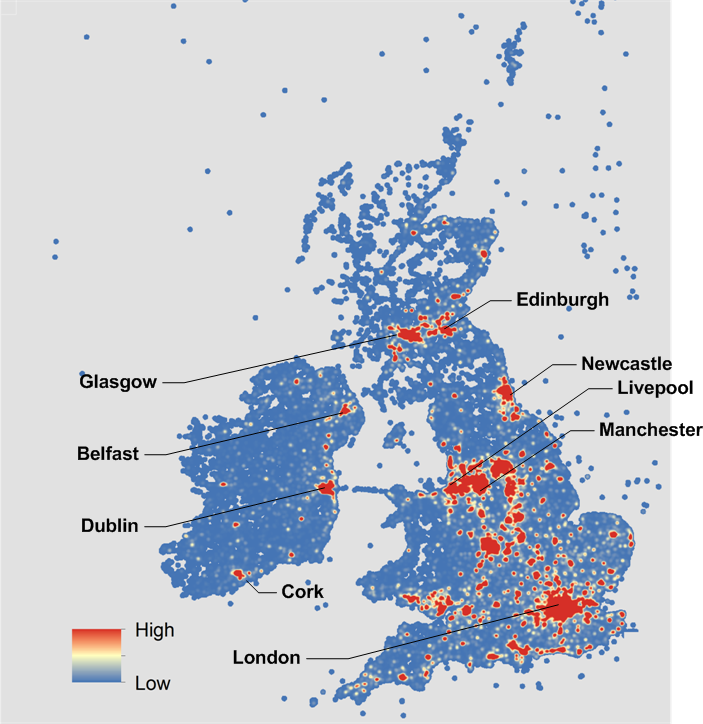
\includegraphics[width=0.8\linewidth]{./figure/S2_twitter_density_Fig_1}
\caption{\bfseries{A density map of the Twitter user locations for July 2014}}
\label{S2_Fig}
\end{center}
\end{figure}

To verify the collected tweets are from human users, the raw tweets were further filtered using the following steps. 
First we removed the duplicated messages in the dataset.
Next, we removed non-human users based on unusual relocation speed \cite{hawelka,jurdak2015}. 
We adopted a relocation speed threshold of 240 m/s as used by \cite{jurdak2015}. 
We examined all of the consecutive locations of each user and excluded those with relocating speeds in excess of the threshold.
Because the original location information embedded in the geo-tag is given in units of latitude and longitude, we projected the points into the British National Grid (EPSG: 27700) coordinate system to reduce the complexity of the required distance calculations. 
Finally, we used the geographical boundary of Great Britain, which is derived from Office for National Statistics (ONS) of UK ({\tt{http://www.ons.gov.uk/ons}}), to further restrict the remaining tweets to be ``domestic".
Based on these restrictions, the filtered dataset for the following study contains 69,847,497 tweets made by 1,153,891 twitter users.

At this stage, each geo-located tweet is represented as a tuple $\langle user\_id, loc, t, m \rangle$, where $user\_id$ is an anonymous Twitter user id; $loc$ is the recorded location of the tweet as a coordinate pair; $t$ is the timestamp of the tweet's post; and $m$ is the actual content of the tweet. 
To protect Twitter user privacy, the id field was replaced with a randomly generated unique number. 
Because we are interested in collective Twitter user movement instead of individual user trajectories, the content of the message was removed. 
Our simplified geo-located tweet dataset can be shared with other researchers upon request.

\subsection{A network of large-scale Twitter user spatial interactions}
Urban regions are discrete urban areas with various socio-economic relationships and citizen commute patterns. 
Some urban regions are more strongly connected to each other than other urban regions.
Therefore, this study connects urban regions when a twitter user's movement begins in one region and ends in another region.
These connections can be represented by an origin-destination (OD) matrix based on the collective Twitter user displacements within the dataset.
This OD matrix is essentially a mathematical representation of a weighted directed graph $G\equiv\langle V, E_{w}\rangle$, where $V$ is a set of spatial nodes corresponding to the underlying urban regions and $E_{w}$ is a set of edges representing the connections between a pair of nodes and the corresponding weights are assigned by the accumulated volume of Twitter user movements.

To build our spatial network at a national level, we had to determine the basic units to serve as spatial nodes of the connectivity network of urban regions.
Previous studies have suggested equi-distant spatial tessellation to generate nodes, which uses voronoi polygons to partition the space based on the collected points~\cite{rinzivillo2012,zhong2014}. 
This approach demonstrates improvements for estimating the locations of mobile phone records based on the cell tower triangulation~\cite{gonzalez2008,qian2013}.
However, equi-distant tessellation decreases the spatial resolution of aggregated geo-located tweets, because the location information is usually derived from the embedded GPS within mobile devices and tends to provide greater accuracy~\cite{sakaki2010,zandbergen2009}.
Another popular approach is to partition the space into a grid of spatial pixels~\cite{liuPopMobility,ratti2010}.
However, the size of the cell can potentially lead to biases due to the Modifiable Area Unit Problem (MAUP)~\cite{openshaw1984,wong2009}, where different choices of unit size can lead to significant variant findings. 
To compare our investigation with the findings of similar studies, and avoid subjectively deciding the cell size, we performed statistical analysis of Twitter user mobility patterns in Great Britain and measured the distribution of collective Twitter user displacements and the radius of gyrations of individuals \cite{gonzalez2008,jurdak2015}.
The radius of gyration is a metric to distinguish mobility patterns of individuals~\cite{gonzalez2008}, which is defined as Eq. \eqref{eq:2}:

\begin{equation} \label{eq:2}
r_{g} = \sqrt{\frac{1}{n}\sum_{i=1}^{n}(p_{i} -  p_{centroid})^{2}}, \textrm{where}\hspace{1ex} p_{centroid} = \frac{1}{n}\sum_{i=1}^{n}p_{i}
\end{equation}

\noindent It measures the accumulated distances of deviation from the center of mass of an individual user's trajectory, where $p_{i}$ is one of the user's locations and $p_{centroid}$ is the center of mass of the user's trajectory.
By examining the probability distributions of the radius of gyration, also known as the spatial dispersal kernel $P(r_g)$~\cite{brockmann2006}, we chose 10 km as the cell size to quantify the spatial coverage of the majority of Twitter users in Great Britain (Fig.~\ref{S4_Fig} - c, with details shown in the next section). 
Thus, we created a fishnet with 2784 10-km size cells.
The cells of the fishnet act as proxies to represent individuals' spatial coverage areas to focus more on the inter-connectivity among cells and identify strongly connected cell clusters. 

\subsection{Community structure of the spatial networks}
Based on the derived spatial network, which is a directed weighted graph, we further determined clusters of strongly connected spatial nodes, known as communities, in the graph space~\cite{coscia2011}. 
There are a variety of community detection algorithms that produce different results depending the definition of community within the network~\cite{coscia2011}.
A common community detection method is based on modularity maximization~\cite{newman2006}, seen in previous studies~\cite{hawelka,ratti2010,song2012}.
However, such an approach is often problematic: it is found to have an inherent resolution problem, where small communities are either ignored~\cite{fortunato2007} or assigned with high modularity scores \cite{guimera2004}; and it is found to produce less informative partitions in many empirical networks~\cite{good2010}.
Since our graph is a directed weighted graph, the alternative community detection library documented in the literature is Infomap~\cite{domenico2015,rosvall2008}, which is considered to produce better community detection results~\cite{lancichinetti2009}.

Infomap uses the map equation~\cite{rosvall2010} to represent the probability of flow of random walks within information systems~\cite{rosvall2008}.
It identifies communities by minimizing the expected description length of the trajectory of a random walker, which is shown below:

\begin{equation} \label{eq:1}
L(M)=qH(Q) + \sum_{i=1}^{m} p_{i}H(p_{i})
\end{equation}

In Eq. \eqref{eq:1} , $L(M)$ consists of two terms: qH(Q) is the entropy of the movement among clusters and $ \sum_{i=1}^{m} p_{i}H(p_{i})$ is the entropy of movement within clusters. 
To be more specific, q is the probability that a random walker jumps from one cluster to another, while $p_i$ is the probability of the in-cluster movement of cluster i.
In this regard, this algorithm can be intuitively tailored to describe strongly connected clusters of urban regions based on Twitter user movement.
The detailed literatures and implementations of Infomap can be found on this website ({\tt{http://mapequation.org}}).
Note that Infomap is capable of performing multi-level community detection~\cite{domenico2015}, but we only use the algorithm to produce our most detailed community structures
to examine groups of strongly connected urban regions.

\section{Results and Discussion}
\subsection{Collective Mobility Patterns of Twitter Users in Great Britain}
We first modeled different aspects of the collective mobility patterns of Twitter users.
These patterns include: the number of visited locations per user,  the collective user displacements, and the radius of gyration of individuals in order to identify natural breaks in user travel patterns.
We then used these natural breaks within the mobility patterns to partition the geographic space of Great Britain into fine-grained cells and established the connectivity among these cells to redraw non-administrative anthropographic urban boundaries. 

We found that the cumulative distribution function~\cite{clauset2009} of the number of locations visited by each Twitter user follows a two-tier power law distribution (shown in Fig.~\ref{S3_Fig}). 
The majority of the data distributed follows a truncated power-law distribution $P(X\geq x)\sim x^{-\alpha}e^{-\lambda x}$, where $\alpha = 1.24, \lambda =0.00132$; and the tail part (less than 2$\%$ of the whole population) follows a power-law distribution  $P(X \geq x)\sim x^{-\alpha}$ with $\alpha$ value is 3.2.
The distribution was found to be consistent over all individual months examined (June to December, 2014), which has a slight offset in the truncated power-law distribution (the mean $\alpha$ value is 1.26 $ \pm$ with a 0.05 $\sigma$ and the mean $\lambda$ value as 0.00134 $ \pm$  with a 0.0002 $\sigma$). 

The two-tier power law distribution indicates that the collective behavior of Twitter users visiting different locations can be well approximated with a (truncated) L\'{e}vy Walk (a random walk) model~\cite{rhee2011,reynolds2012}, which has also been identified in many human mobility studies using different mobility data~\cite{zhao2015}.
The similarity among the distributions suggests that the mobility data collected from geo-located tweets is temporally stable, at least at the monthly interval, which indicates that our approach using Twitter user mobility to delineate urban boundaries is viable.  
In addition, the L\'{e}vy Walk model reveals the diversity regarding the number of visited locations per user, which indicates a level of ``randomness'' in Twitter user movement across space. 
It, in turn, justifies our choice of using the map equation community detection algorithm~\cite{rosvall2008} to identify the clusters of urban regional connectedness using large-scale Twitter user movement data.


\begin{figure}[ht]
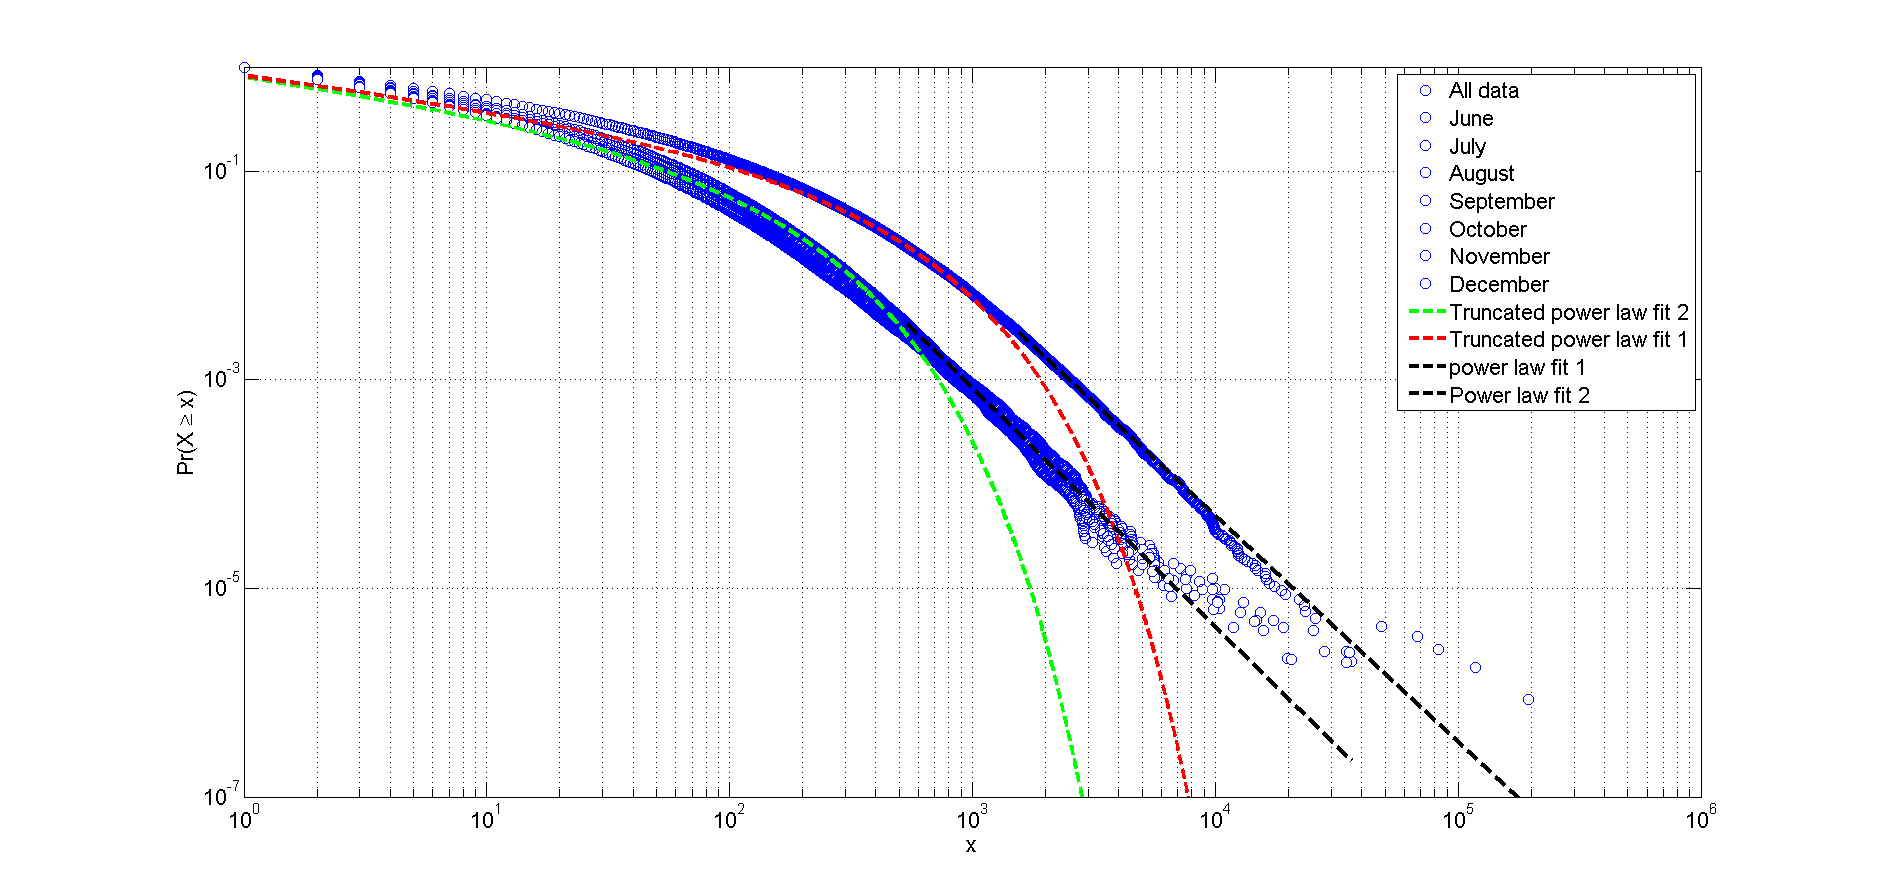
\includegraphics[width=1.0\linewidth]{./figure/S3_visitation}
\caption{ \bfseries{Cumulative distribution of the number of locations visited by each Twitter user during different timespan}}
\label{S3_Fig}
\end{figure}

We further studied two aspects of the Twitter user mobility patterns: the distribution of Twitter user displacement and the radius of gyration. 
Twitter user displacement refers to the distance between two consecutive locations in a user's trajectory using a straight-line distance metric.
The radius of gyration describes the deviation of distance from the center of mass in a user's trajectory.
The probability distributions of the collective user displacement $P(d)$ and radius of gyration $P(r_g)$ are presented in Fig.~\ref{S4_Fig}, where the fitting method for identifying different distance ranges is derived from~\cite{jurdak2015}.
The probability distribution of the collective displacements can be approximated by $P(d) \sim \lambda_{1} e^{-\lambda_{1}(d - d_{min})}, d_{min}=10m$ from [10m, 70m] (accounting for 3 $\%$ of the population),  $ P(d) \sim \beta\lambda_{1}d^{\beta-1}e^{-\lambda^{1}(d^\beta-d_{min}^\beta)}, d_{min} = 100m$ from [70m, 70km] (93 $\%$ of the population), and $P(d) \sim {d}^{-\alpha}$ [$>$ 70km] (4 $\%$ of the population). 
The displacement distance between 70m and 100km can be further approximated by two power law distributions with a cut-off point at 4km (55$\%$ distances are less than 4km and 40$\%$ distances between 4km and 100km), which indicates the urban movement captured by the geo-located Twitter data to reveal two different modes: inter-city and intra-city movement. 
In short, these fitting functions suggest the existence of multi-scale or multi-modal urban movements captured from Twitter users in Great Britain, which means the geographically cohesive, non-overlapping urban areas identified in the next section are not just a result of short distance movement but emerge naturally from the broader Twitter user mobility pattern.
Note that a similar multiphase pattern was observed in Twitter user displacements in Australia, but with slightly different distance ranges\cite{jurdak2015}.

Further, we analyzed the distribution of radius of gyration to understand the movement from the point of view of individual Twitter users rather than separate displacements.
The distribution of the radius of gyration can be approximated through a combination of three functions: $P(r_{g}) \sim \lambda_{2} e^{-\lambda_{2}(r_{g} - {r_{g}}_{min})}, {r_{g}}_{min}=10m$ from [10 m, 30m], $P(r_{g}) \sim \lambda_{2} e^{-\lambda_{2}(r_{g} - {r_{g}}_{min})}$ from [50m, 10km], and $P(r_{g}) \sim {r_{g}}^{-\alpha}$ [10km, 100km], where these three functions account for 92$\%$ of all the users.
This suggests that there are three primary types of users that: (1) tend to stay at one location or at nearby locations when they tweet, or (2) tend to move at the intra-city scale when they tweet, or (3)  tend to exhibit a large spatial coverage. 
(1) and (2) account for approximately 53$\%$ of all users.  
The radius of gyration between 30m and 100km can be further approximated by two power law distributions with a cut-off point at 2.5km (35 $\%$ users with radius of gyration less than 2.5km and 57$\%$ users with radius of gyration between 3km and 100km) that suggests two main types of spatial coverage of Twitter user movement within 
Great Britain. 
Note that the accuracy of these values for defining the distance bound depends upon the accuracy of the location information of each geo-located tweet. 
These findings are consistent with the findings in the literature on human mobility, where the radius of gyration of human movement is bounded to different distance ranges~\cite{brockmann2006,gonzalez2008}.
The distance-decay effects found in both user displacements and the radius of gyration shows evidence of spatial proximity in Twitter user movement. 
It explains that the communities of urban regions within the graph space are geographically close, but are able to be separated from other groups, which results in the delineation of urban boundaries based on the spatial interactions of Twitter users.


\begin{figure}[ht]
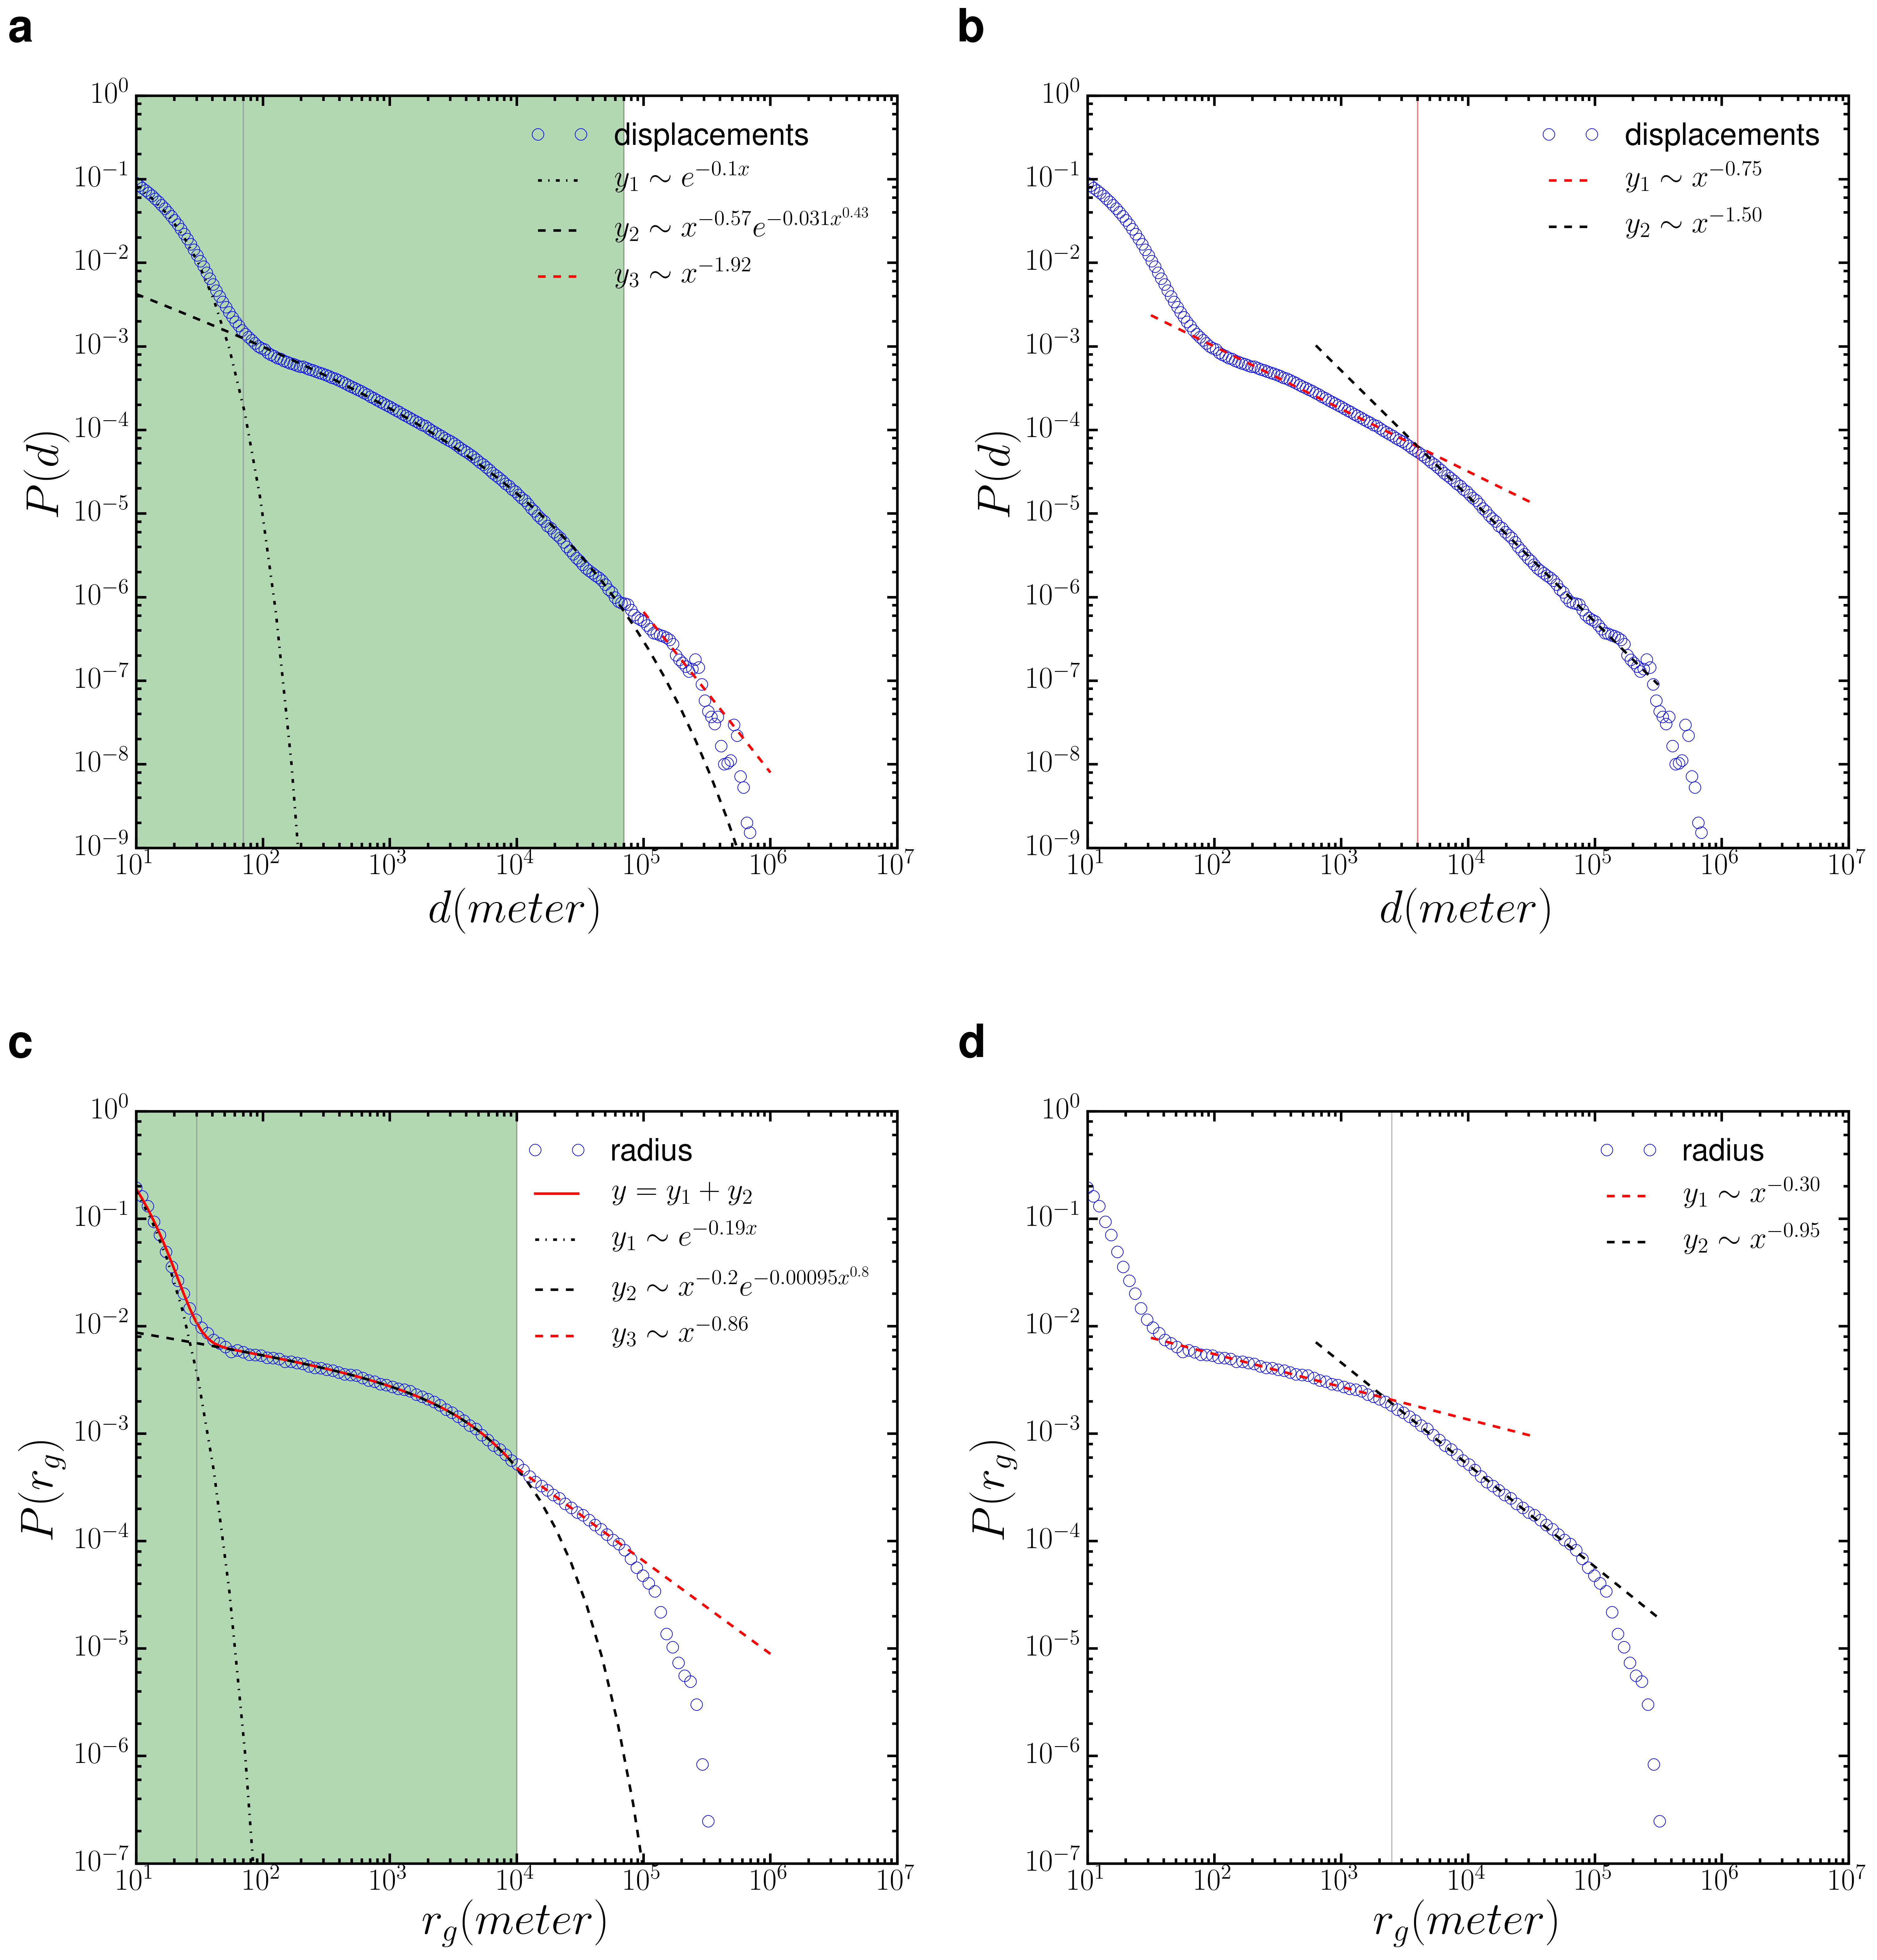
\includegraphics[width=1.0\linewidth]{./figure/S4_radius_displacement}
\caption{{\bf The probability distribution of Twitter user displacements and radius of gyration:} (a) The displacement distribution $P(d)$ is approximated by an exponential, a stretched-exponential and a power-law function (b) the distance between [70m, 70km] is approximated by a double power-law functions (c) The distribution of radius of gyration $P(r_g)$ is approximated by the combination of an exponential, a stretched-exponential and a power-law function (d) the distance between [30m, 100 km] is approximated by a double power-law functions}
\label{S4_Fig}
\end{figure}

\subsection{Redrawing Great Britain’s Urban Boundaries}
The network of Twitter user spatial interaction was constructed by nodes representing 10 km by 10 km fishnet cells that provide an adequate resolution for a country wide investigation~\cite{ratti2010}.
The edges of this network were derived from the number of directed Twitter user displacements between each pair of cells.
We used this connectivity network as a proxy to partition the space associated with its nodes.
Coherent geographic regions were identified as individual fishnet cells showing more internal user movement compared to user movements across the cell boundaries to neighboring cells.
Fig.~\ref{S5_Fig}  presents the delineated urban boundaries based on Twitter user displacement distance less than 4 km, greater than 4km, greater than 10 km, and using all available displacements together compared to the administrative boundaries of Great Britain.
One clear observation across the coarse and fine delineations is that most of the geographic divisions are centered around big urban cores with relatively high populations.
These results are expected given that most of the tweets originate in urban centers.
However, what is remarkable is the performance of this approach in dividing the remaining space between cities.
We found that restricting the trip distance results in different delineations of the catchment area around these centers.
For example, one could explain these effects as a manifestation of the underlying gravity law~\cite{simini2012} and the distance decay effect on attracting movers~\cite{gonzalez2008}.
Remarkably, our approach performed well in terms of dividing the entire space with minimum gaps.
Empty cells were found in regions where no, or few, Twitter users had visited (e.g. forests, agriculture) especially when restricting the analysis to short distance Twitter user displacements.

\begin{figure}[ht]
\begin{center}
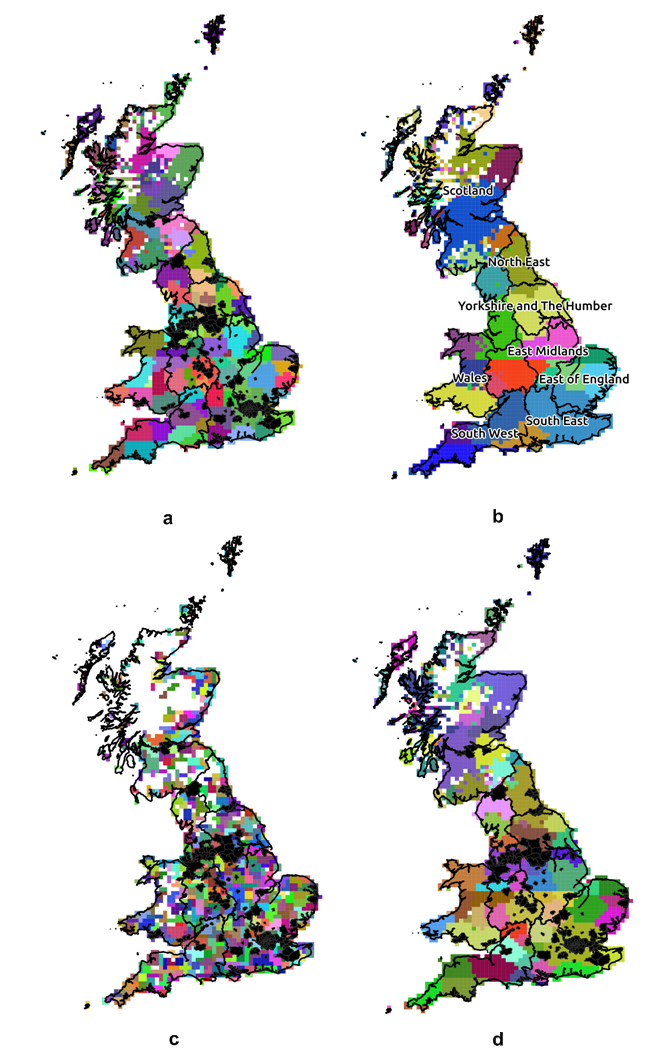
\includegraphics[width=0.9\linewidth]{./figure/S5_community}
\caption{{\bf The community structure from collective Twitter user displacements reveals non-administrative anthropographic urban boundaries} (a) displacements longer than 10 km (b) displacements shorter than 4 km (c) and displacements longer than 4 km (d) The partition of space was done using a 10 km fishnet to map the directed displacements from and to each cell. Each color represents a unique community with more Twitter users displacements among the cells compared to others. Major cities (urban audit functional areas) and NUTS are displayed in black.}
\label{S5_Fig}
\end{center}
\end{figure}

Regional boundaries inferred from short distance Twitter user displacements (less than 4 km) exhibit very small and fragmented regions, which is probably related to daily commuting around a user's home location. 
Redrawing the boundaries based on longer distance displacements produces more cohesive, large regions.
For example, by partitioning the space based on displacements greater than 10 km created regions that are comparable to the NUTS (Nomenclature of Territorial Units for Statistics - 1) regions (Fig.~\ref{S6_Fig} - a). 
However, the power of this novel mapping technique is not to reproduce the partitions already known, rather it is to point out some of the unexpected boundaries.
For example the boundaries between England and Wales were found to be more diffuse compared to the abrupt boundary of England and Scotland.
Moreover, the city of London has a wider visitor catchment area that extends beyond the authoritative boundaries of the city.
Increasing the displacement distance results in revealing the large region connected to London (Fig.~\ref{S6_Fig}). 

Using Twitter user mobility to delineate non-administrative anthropographic boundaries enables the researcher to redraw the city at different mobility ranges inferred objectively from the user's collective distribution. 
In addition, the distance range of the movements is usually explained by local socio-economic factors (e.g., work commuting ) that provide for a specific interpretation of the apparent patterns.
The patterns obtained from Twitter user mobility are comparable to the patterns produced by those of the network of landline phone calls~\cite{ratti2010}.\
For example, the region of Wales appears to consist of three communities as found in the connectivity of both phone calls and long distance movements. 
However, the regions extracted from the mobility network seems to be more spatially consistent with minimal spatial gaps compared to the partitions extracted from land-line call networks in Great Britain~\cite{ratti2010}.

\begin{figure}[ht]
\begin{center}
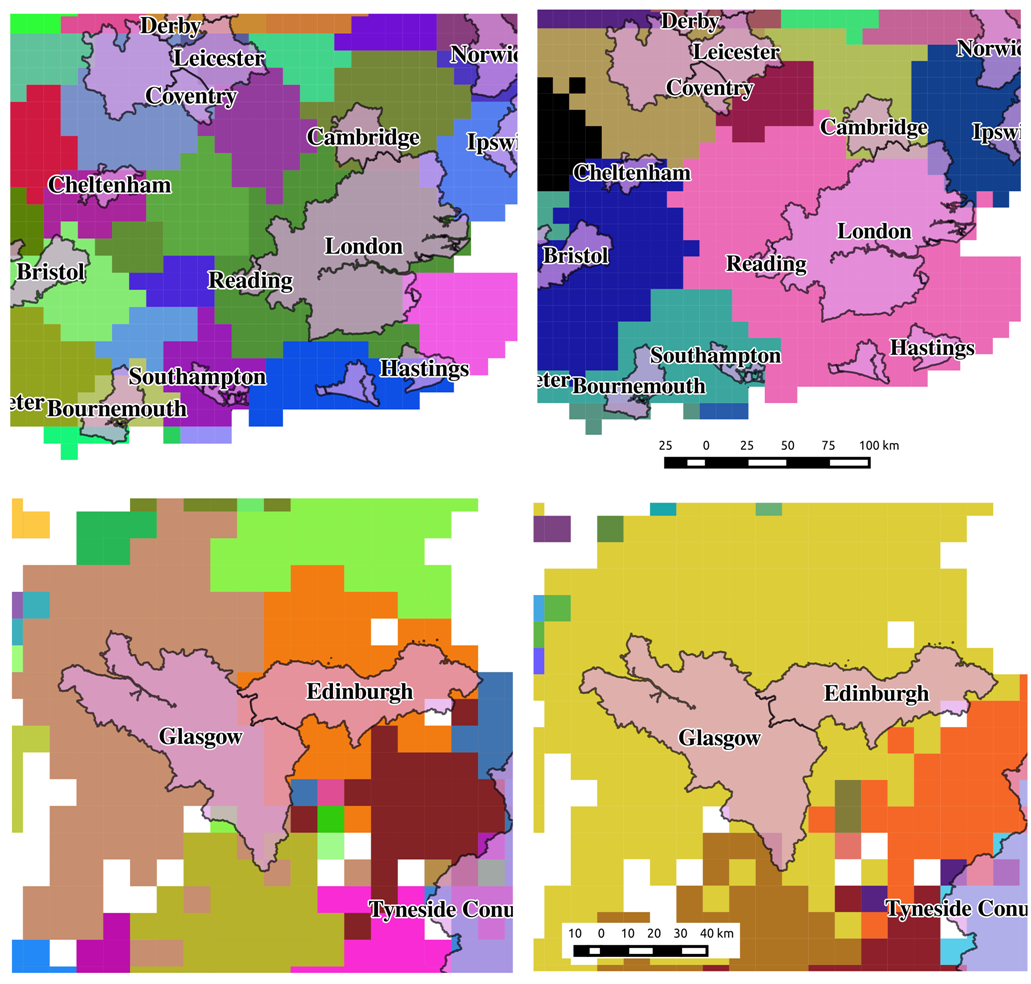
\includegraphics[width=0.7\linewidth]{./figure/S6_community_london}
\caption{{\bf The non-administrative anthropographic regions inferred from Twitter user displacements greater than 4 km (left) and 10 km (right) in comparison with major cities in England (upper figures) and Scotland (bottom figures).}  Each color represents a unique community. Including short distance movements has increased the power to differentiate the influence of nearby cities such as Glasgow and Edinburgh (lower left), while restricting the analysis to longer distance movements grouped travelers from the two previous cities into the same community (lower right).}
\label{S6_Fig}
\end{center}
\end{figure}

A more detailed study was conducted over the greater London region revealing the intra-city spatial interaction patterns.
The spatial partitions derived from a fine grid of 1km using all available Twitter user trips without any restriction on trip distances yields geographic boundaries comparable to some of London's boroughs  (Fig.~\ref{S7_Fig}).
However, some areas are shown to be more cohesive and display greater spatial interactions across the administrative boundaries, for instance, central London.
Although, these results suggest that travelers seem to be localized over certain areas of the city most of the time, some regions do exhibit long distance interaction patterns.
For example, the separate geographic areas in the south of Hillingdon which includes Heathrow Airport exhibits more connectivity to central London than its surrounding areas, which is explained by the usual flight passenger routes.
The technique also reveals some of the emerging communities around the borders due to the spatial intermingling of both communities.
For example, East Barnet and West Enfield seem to have higher interactions than those resulted from in the emerging cohesive zone between the two boroughs.

\begin{figure}[ht]
\begin{center}
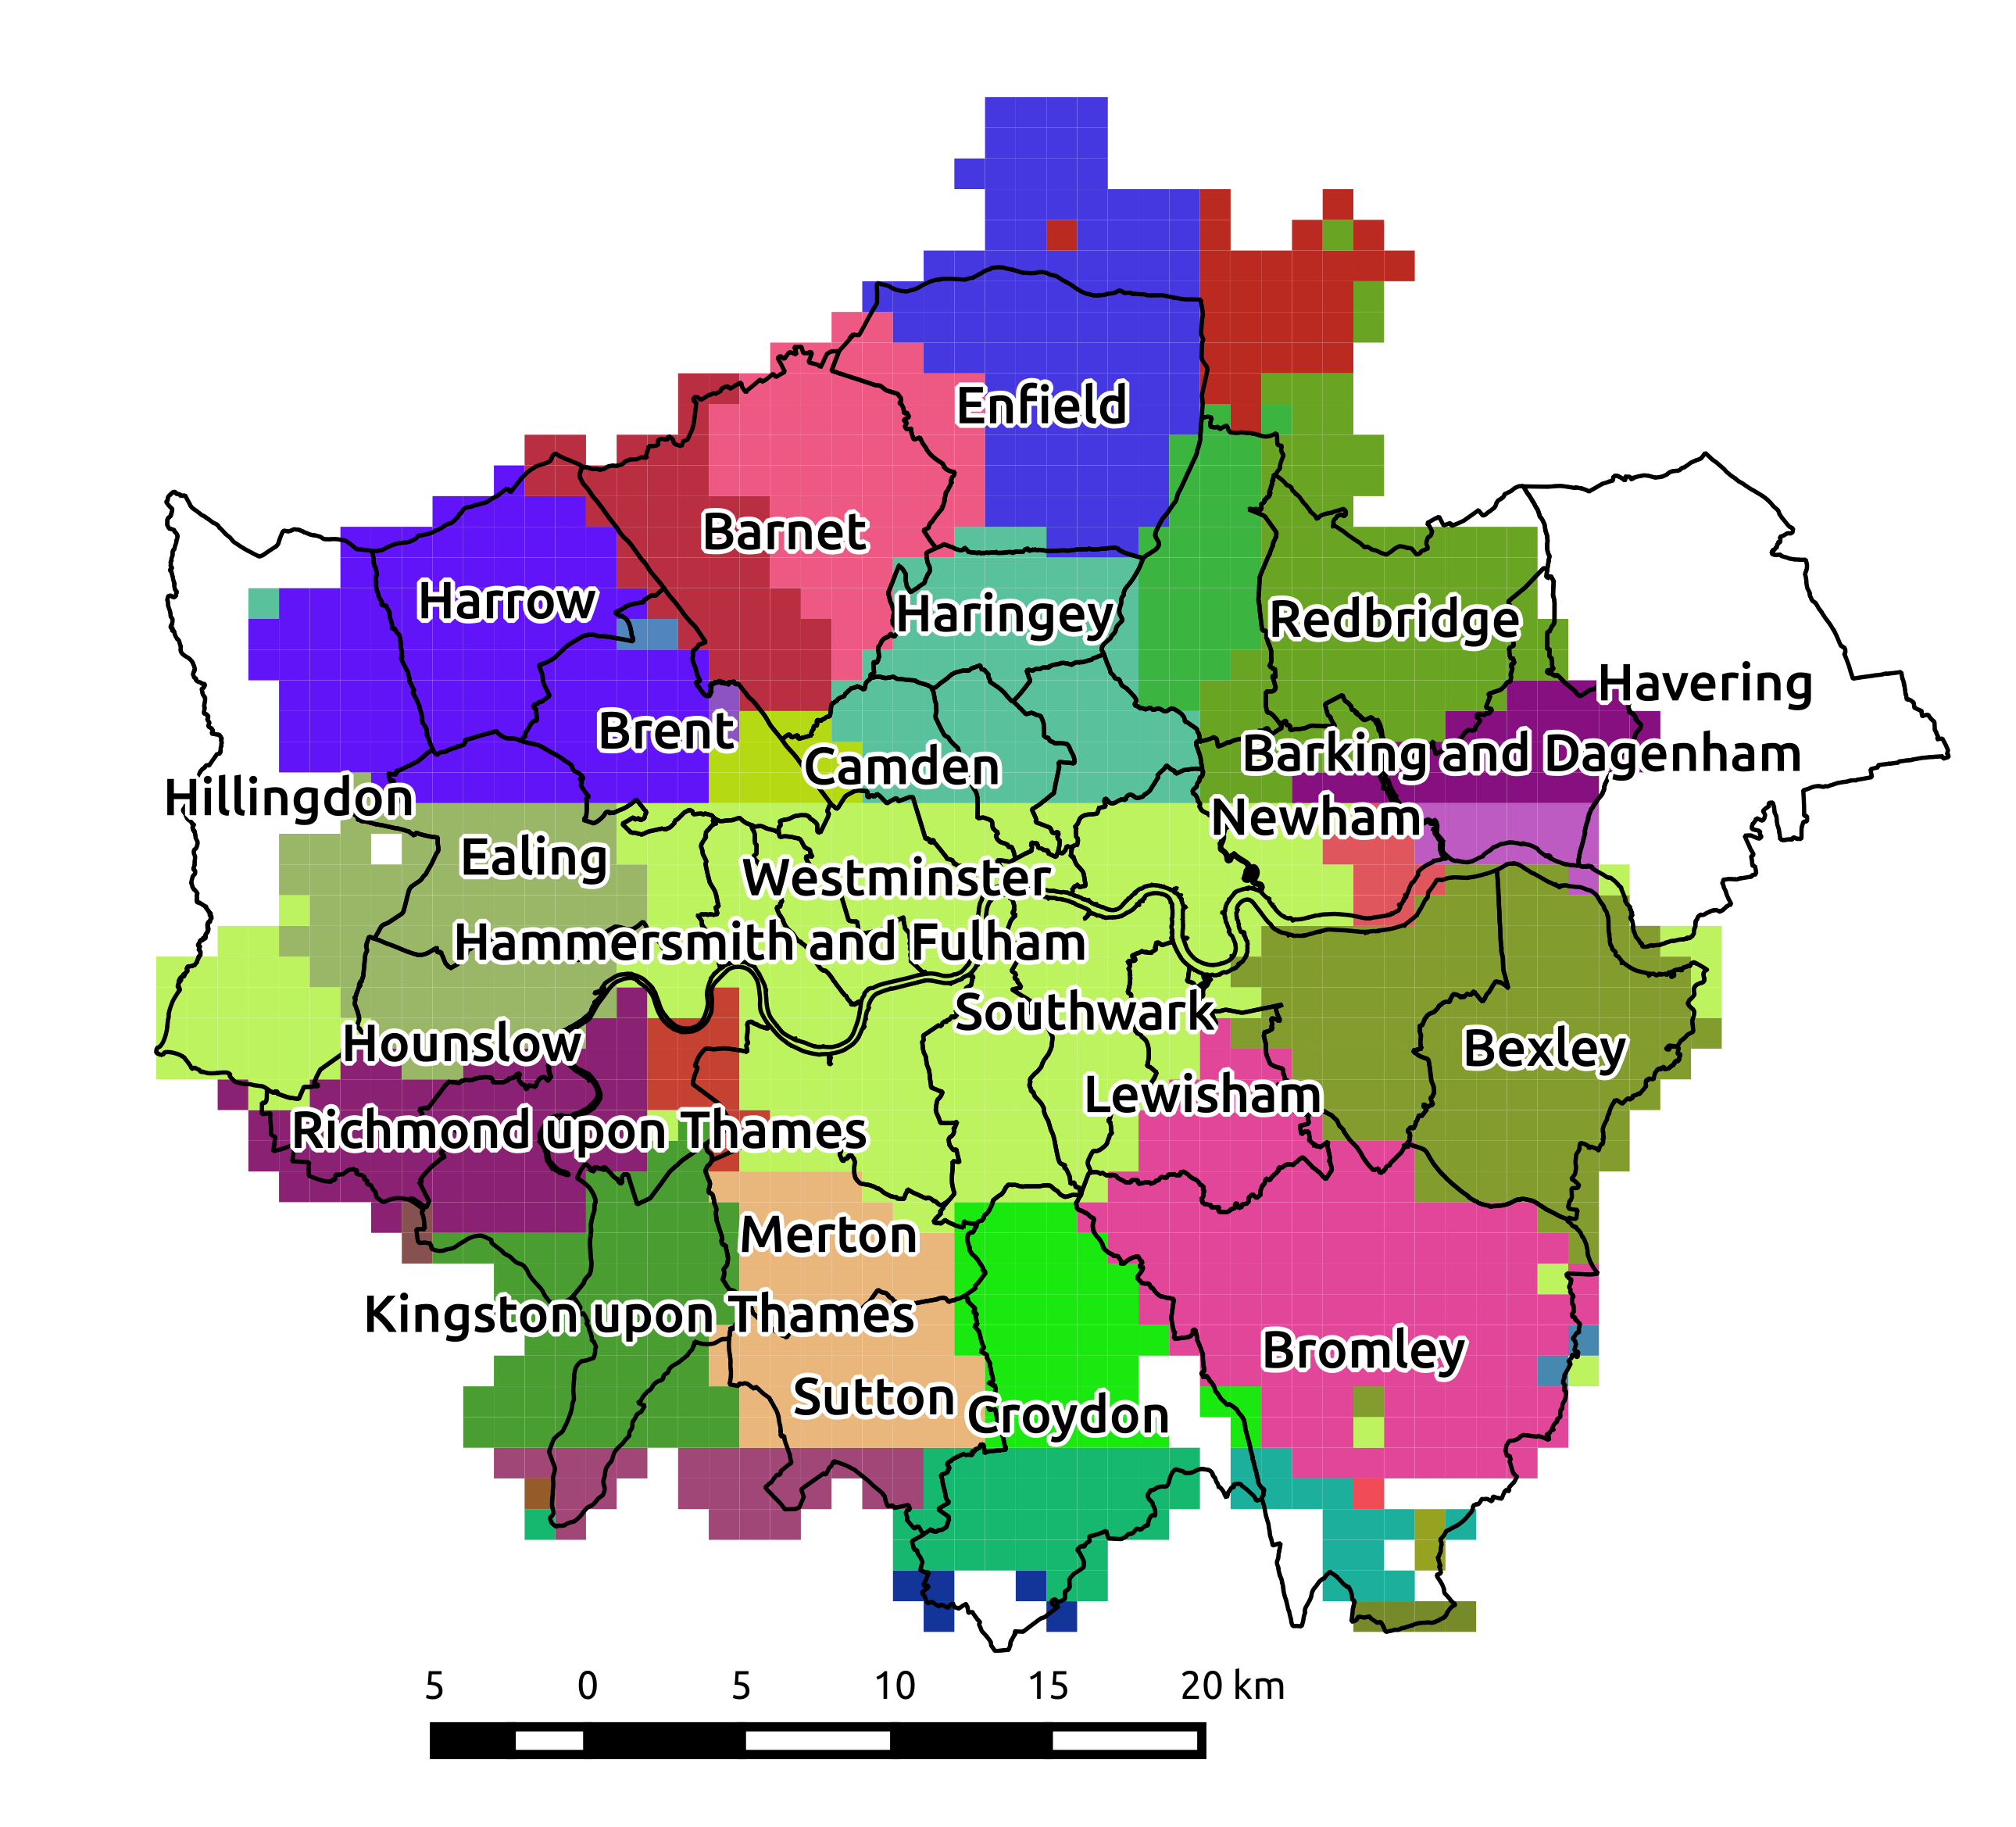
\includegraphics[width=0.8\linewidth]{./figure/S7_london}
\caption{{\bf Non-administrative anthropographic boundaries inferred from collective Twitter user displacements in the city of London compared to the boundaries of London boroughs}  A fine fishnet of 1 km cells were used to identify the detailed connectivity patterns based on all the Twitter user displacements in the area.  Each unique color represents a different non-administrative anthropographic region. Notice that some remote regions like the airport (light green region in south of Hillingdon) share the same class with downtown because it is well connected despite the geographic separation.}
\label{S7_Fig}
\end{center}
\end{figure}

\clearpage
\section{Conclusion}
In this study, we delineated the non-administrative anthropographic urban boundaries in Great Britain using a network of Twitter user spatial interactions, which were inferred from the collective Twitter user movement data extracted from more than 69 million Twitter messages.
In contrast to administrative urban boundaries, our ``bottom-up" approach imposes a virtual fishnet over the islands of Great Britain to partition the space.
By studying the probability distributions of the radius of gyrations of individual Twitters users, we selected a cell size of 10 km to quantify the spatial coverage of the majority of Twitter users in Great Britain. 
Twitter user movements were used to establish a connectivity network of the fishnet cells.
Then we applied the map equation algorithm to partition the network and associated geographic regions.
The strongly connected communities within the network space yields geographically cohesive, non-overlapping urban areas that provides a clear delineation of the urban boundaries in Great Britain.
By performing a statistical analysis of Twitter user mobility patterns in Great Britain, in particular the distribution of collective Twitter user displacements, we found multi-scale and multi-modal urban movements that were divided into several distance ranges starting from short intra-city to inter-city movements with clear destination points.
Identifying the connected regions at each of these distance ranges yielded hierarchical boundaries of  the urban space in Great Britain.

The power of using Twitter user mobility to delineate non-administrative anthropographic boundaries is the ability to redraw the city at different mobility ranges inferred objectively from the collective mobility patterns. 
Urban boundaries redrawn based on Twitter user movement represent physical commutes rather than social ties or phone call initiation to reflect the human interaction space.
This study provides a first step in connecting human mobility research with defining non-administrative anthropographic boundaries, which could assist in resource allocation, political campaigns and urban planning. However, the geo-located twitter data is not able to generalize to the entire population; therefore, the urban regions that do not have any, or limited, Twitter coverage can be missed during the delineation process. Yet, our approach is still applicable when more detailed mobility data is available. 

%\subsection{Acknowledgements}


\begin{thebibliography}{9}

\markboth{International Journal of Geographical Information Science}{International Journal of Geographical Information Science}

\bibitem[\protect\citeauthoryear{Brockmann {\itshape{et~al.}}}{2006}]{brockmann2006}
Brockmann, D., Hufnagel, L., Geisel, T., 2006. The scaling laws of human travel. Nature 439, 462–5. doi:10.1038/nature04292

\bibitem[\protect\citeauthoryear{Clauset {\itshape{et~al.}}}{2009}]{clauset2009}
Clauset, A., Shalizi, C., Newman, M., 2009. Power-Law Distributions in Empirical Data. Society for Industrial and Applied Mathematics Review. 51, 661–703. doi:10.1137/070710111

\bibitem[\protect\citeauthoryear{Coscia {\itshape{et~al.}}}{2011}]{coscia2011}
Coscia, M., Giannotti, F., Pedreschi, D., 2011. A Classification for Community Discovery Methods in Complex Networks. Statistical Analysis and Data Mining, 4, 512–546. doi:10.1002/sam.10133


\bibitem[\protect\citeauthoryear{De Domenico {\itshape{et~al.}}}{2015}]{domenico2015}
De Domenico, M., Lancichinetti, A., Arenas, A., Rosvall, M., 2015. Identifying Modular Flows on Multilayer Networks Reveals Highly Overlapping Organization in Interconnected Systems. Physical Review X, 5. doi:10.1103/PhysRevX.5.011027

\bibitem[\protect\citeauthoryear{Fortunato and Barthélemy}{2007}]{fortunato2007}
Fortunato, S., Barthélemy, M., 2007. Resolution limit in community detection. Proceedings of the National Academy of Sciences, 104, 36–41. doi:10.1073/pnas.0605965104

\bibitem[\protect\citeauthoryear{González {\itshape{et~al.}}}{2008}]{gonzalez2008}
González, M.C., Hidalgo, C.A., Barabási, A.-L., 2008. Understanding individual human mobility patterns. Nature, 453, 779–82. doi:10.1038/nature06958


\bibitem[\protect\citeauthoryear{Good {\itshape{et~al.}}}{2010}]{good2010}
Good, B.H., de Montjoye, Y.-A., Clauset, A., 2010. Performance of modularity maximization in practical contexts. Physical Review E, 81, 046106. doi:10.1103/PhysRevE.81.046106

\bibitem[\protect\citeauthoryear{Guimerà {\itshape{et~al.}}}{2004}]{guimera2004}
Guimerà, R., Sales-Pardo, M., Amaral, L.A.N., 2004. Modularity from fluctuations in random graphs and complex networks. Physical Review E, 70, 025101. doi:10.1103/PhysRevE.70.025101

\bibitem[\protect\citeauthoryear{Hawelka {\itshape{et~al.}}}{2014}]{hawelka}
Hawelka, B., Sitko, I., Beinat, E., Sobolevsky, S., Kazakopoulos, P., Ratti, C., 2014. Geo-located Twitter as proxy for global mobility patterns. Cartography and Geographic Information Science, 41, 260–271. doi:10.1080/15230406.2014.890072


\bibitem[\protect\citeauthoryear{Jiang and Miao}{2015}]{jiang2015}
Jiang, B., Miao, Y., 2015. The evolution of natural cities from the perspective of location-based social media. The Professional Geographer, 67(2), 295-306.

\bibitem[\protect\citeauthoryear{Jurdak {\itshape{et~al.}}}{2015}]{jurdak2015}
Jurdak, R., Zhao, K., Liu, J., AbouJaoude, M., Cameron, M., Newth, D., 2015. Understanding Human Mobility from Twitter. PLoS ONE 10, e0131469. doi:10.1371/journal.pone.0131469


\bibitem[\protect\citeauthoryear{Kallus {\itshape{et~al.}}}{2015}]{kallus2015}
Kallus Z, Barankai N, Szüle J, Vattay G., 2015. Spatial Fingerprints of Community Structure in Human Interaction Network for an Extensive Set of Large-Scale Regions. PLoS ONE 10(5): e0126713. doi: 10.1371/journal.pone.0126713 


\bibitem[\protect\citeauthoryear{Lancichinetti and Fortunato}{2009}]{lancichinetti2009}
Lancichinetti, A., Fortunato, S., 2009. Community detection algorithms: A comparative analysis. Physical Review E, 80, 056117. doi:10.1103/PhysRevE.80.056117


\bibitem[\protect\citeauthoryear{Liu {\itshape{et~al.}}}{2015}]{liu2015}
Liu, X., Gong, L., Gong, Y., Liu, Y., 2015. Revealing travel patterns and city structure with taxi trip data. J. Transportation Geography, 43, 78–90. doi:10.1016/j.jtrangeo.2015.01.016

\bibitem[\protect\citeauthoryear{Liu {\itshape{et~al.}}}{2014}]{liuPopMobility}
Liu, J., Zhao, K., Khan, S., Cameron, M., Jurdak, R., 2014. Multi-scale Population and Mobility Estimation with Geo-tagged Tweets. ArXiv14120327 Phys.


\bibitem[\protect\citeauthoryear{Long {\itshape{et~al.}}}{2015}]{long2015}
Long, Y., Han, H., Tu, Y., Shu, X., 2015. Evaluating the effectiveness of urban growth boundaries using human mobility and activity records. Cities, 46, 76-84.

\bibitem[\protect\citeauthoryear{Lynch}{1960}]{lynch1960}
Lynch, K., 1960. The image of the city. MIT press.





\bibitem[\protect\citeauthoryear{Newman}{2006}]{newman2006}
Newman, M.E.J., 2006. Modularity and community structure in networks. Proceedings of the National Academy of Sciences, 103, 8577–82. doi:10.1073/pnas.0601602103





\bibitem[\protect\citeauthoryear{Openshaw}{1984}]{openshaw1984}
Openshaw, S., 1984. The modifiable areal unit problem. Geo Abstracts University of East Anglia.



\bibitem[\protect\citeauthoryear{Qian {\itshape{et~al.}}}{2013}]{qian2013}
Qian, W., Stanley, K. G., Osgood, N. D., 2013. The impact of spatial resolution and representation on human mobility predictability. In Web and Wireless Geographical Information Systems,  pp. 25-40, Springer Berlin Heidelberg.

\bibitem[\protect\citeauthoryear{Ratti {\itshape{et~al.}}}{2010}]{ratti2010}
Ratti, C., Sobolevsky, S., Calabrese, F., Andris, C., Reades, J., Martino, M., Claxton, R., Strogatz, S.H., 2010. Redrawing the Map of Great Britain from a Network of Human Interactions. PLoS ONE 5, e14248. doi:10.1371/journal.pone.0014248


\bibitem[\protect\citeauthoryear{Reynolds}{2012}]{reynolds2012}
Reynolds, A., 2012. Truncated levy walks are expected beyond the scale of data collection when correlated random walks embody observed movement patterns. Journal of The Royal Society Interface, 9(68), 528-534.



\bibitem[\protect\citeauthoryear{Rhee {\itshape{et~al.}}}{2011}]{rhee2011}
Rhee, I., Shin, M., Hong, S., Lee, K., Kim, S. J., and Chong, S., 2011. On the levy-walk nature of human mobility. IEEE/ACM transactions on networking (TON), 19(3), 630-643.

\bibitem[\protect\citeauthoryear{Rinzivillo {\itshape{et~al.}}}{2012}]{rinzivillo2012}
Rinzivillo, S., Mainardi, S., Pezzoni, F., Coscia, M., Pedreschi, D., Giannotti, F., 2012. Discovering the Geographical Borders of Human Mobility. KI - Künstl. Intell. 26, 253–260. doi:10.1007/s13218-012-0181-8


\bibitem[\protect\citeauthoryear{Rosvall {\itshape{et~al.}}}{2010}]{rosvall2010}
Rosvall, M., Axelsson, D., Bergstrom, C.T., 2010. The map equation. The European Physical Journal Special Topics, 178, 13–23. doi:10.1140/epjst/e2010-01179-1

\bibitem[\protect\citeauthoryear{Rosvall and Bergstrom}{2008}]{rosvall2008}
Rosvall, M., Bergstrom, C.T., 2008. Maps of random walks on complex networks reveal community structure. Proceedings of the National Academy of Sciences, 105, 1118–1123.





\bibitem[\protect\citeauthoryear{Sakaki {\itshape{et~al.}}}{2010}]{sakaki2010}
Sakaki, T., Okazaki, M., Matsuo, Y., 2010. Earthquake Shakes Twitter Users: Real-time Event Detection by Social Sensors, in: Proceedings of the 19th International Conference on World Wide Web, WWW ’10. ACM, New York, NY, USA, pp. 851–860. doi:10.1145/1772690.1772777




\bibitem[\protect\citeauthoryear{schliephake}{2014}]{schliephake}
Schliephake, C., 2014. Urban Ecologies: City Space, Material Agency, and Environmental Politics in Contemporary Culture. Lexington Books.

\bibitem[\protect\citeauthoryear{Simini {\itshape{et~al.}}}{2012}]{simini2012}
Simini, F., González, M. C., Maritan, A., Barabási, A. L., 2012. A universal model for mobility and migration patterns. Nature, 484(7392), 96-100.

\bibitem[\protect\citeauthoryear{Sobolevsky {\itshape{et~al.}}}{2013}]{sobolevsky2013}
Sobolevsky S, Szell M, Campari R, Couronné T, Smoreda Z, Ratti, C., 2013. Delineating Geographical Regions with Networks of Human Interactions in an Extensive Set of Countries. PLoS ONE 8(12): e81707. doi: 10.1371/journal.pone.0081707


\bibitem[\protect\citeauthoryear{Song {\itshape{et~al.}}}{2012}]{song2012}
Song, C., Wang, D., Barabási, A.-L., 2012. Connections between human dynamics and network science. ArXiv Prepr. ArXiv12091411.


\bibitem[\protect\citeauthoryear{Thiemann {\itshape{et~al.}}}{2010}]{thiemann}
Thiemann, C., Theis, F., Grady, D., Brune, R., Brockmann, D., 2010. The Structure of Borders in a Small World. PLoS ONE 5, e15422. doi:10.1371/journal.pone.0015422



\bibitem[\protect\citeauthoryear{Wong}{2009}]{wong2009}
Wong, D., 2009. The modifiable areal unit problem (MAUP). SAGE Publications: London, UK.

\bibitem[\protect\citeauthoryear{Zandbergen}{2009}]{zandbergen2009}
Zandbergen, P.A., 2009. Accuracy of iPhone Locations: A Comparison of Assisted GPS, WiFi and Cellular Positioning. Transactions in GIS, 13, 5–25. doi:10.1111/j.1467-9671.2009.01152.x


\bibitem[\protect\citeauthoryear{Zhao {\itshape{et~al.}}}{2015}]{zhao2015}
Zhao, K., Musolesi, M., Hui, P., Rao, W., and Tarkoma, S., 2015. Explaining the power-law distribution of human mobility through transportation modality decomposition. Scientific reports, 5.

\bibitem[\protect\citeauthoryear{Zhong {\itshape{et~al.}}}{2014}]{zhong2014}
Zhong, C., Arisona, S.M., Huang, X., Batty, M., Schmitt, G., 2014. Detecting the dynamics of urban structure through spatial network analysis. International Journal of Geographical Information Science, 28, 2178–2199. doi:10.1080/13658816.2014.914521

\end{thebibliography}

\bibliographystyle{tGIS}
%\bibliography{Twitter_Urban_Boundary}




\label{lastpage}

\end{document}
